%!TEX root = doc.tex
\section{Verification}
\label{sec:verification}



To perform the verification of the API, we developed a contract net scenario. This was a deterministic test which used a fixed data set, thus having always having the same outcome. The example was implemented in Repast and then manually ported to JADE, after some adaptations.

\subsection{Experiment Setup}

The diagram in Figure \ref{fig:CNetExample} tries to illustrate the contract net created for this test. An agent - the buyer - intends to purchase a certain quantity of three kinds of goods - rice, flour and oats. Besides the quantities of each product it needs, the buyer also stipulates a maximum price for the whole deal. The buyer will issue a call for proposals (CFP) containing a request for supplies to all agents that announce themselves as suppliers.

The supplier agents have a maximum supply capacity and a price for each product. After receiving a CFP, the supplier will send a price proposal to the buyer if the supply is within the seller's capacity. Otherwise, a REFUSE message will be sent to the buyer.

Finally, the buyer agent will compare all valid proposals, choose the cheapest offer and send an ACCEPT PROPOSAL to the owner of the best offer, and REJECT PROPOSAL to every other agent.

\begin{figure}[h]
	\centering
	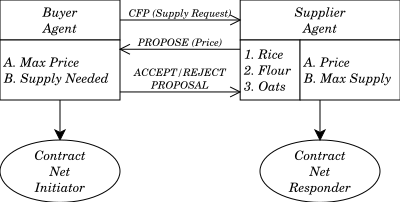
\includegraphics[width=3.0in]{figures/CNetExample.pdf}
	\caption{
		Representation of the example contract net.
	}
	\label{fig:CNetExample}
\end{figure}

Using a large data set with values for prices and supply capacity in both frameworks, we ensured the proper comparison of results. For demonstration purposes, we focused on two simple metrics to evaluate our work: time and  outcome.

The time was measured from be begining of the protocol, until all suppliers were notified. The JADE application was also tested in two different setups: first, with all agents running in a single container; second, with the supplier agents in one container and the buyer in a separate one (but in the same machine). All tests were performed using an Intel i7 CPU (8 logical cores). The second validation metric we used was the actual result of the protocol, i.e who was the supplier agent chosen by the buyer and its price proposal.

\subsection{Results}

The average performance on both experiments is represented in \ref{fig:performance}. As excepted, Repast excels when the number of agents is high. JADE was able to perform better with a lower number of agents by taking advantage of its multi-threaded architecture - more so when using two distinct containres. As studied by Mengistu et. al \cite{mengistu2008scalability}, JADE's performance drops very significantly when there is a high communication-to-computation ratio in the application.

Regarding the outcome of the protocol, an equal value was obtained in the three experiments with equal number of agents. This allowed us to verify that the behaviour of the protocol was similar identical in both implementations.


%%%%%%%%%%%%%%%%%%%%%%%%%%%%%%%%%%%%%%%%%%%%%%%
%%%%%%%%%%%%%%%%%% The Chart %%%%%%%%%%%%%%%%%%

\begin{figure}[h]
	\centering
	%\includegraphics[width=\linewidth]{figures/performance.png}
	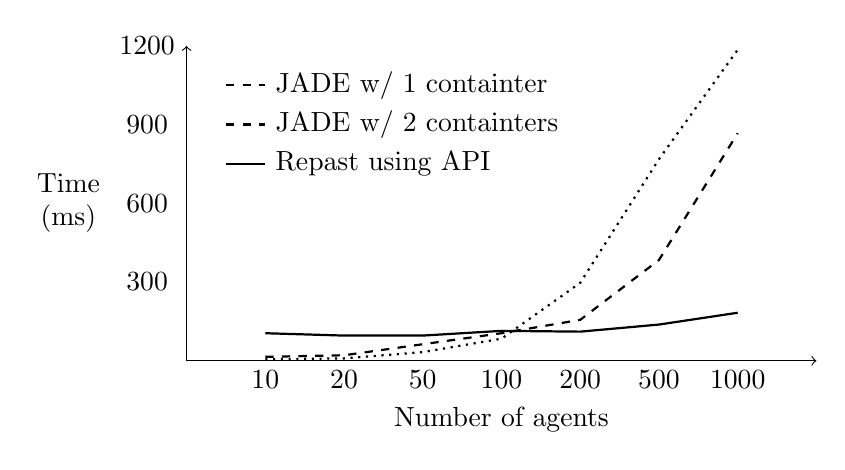
\begin{tikzpicture}

		% horizontal axis
		\draw[->] (0,0) -- (8,0);
		\draw (4,-0.75) node[align=center] {Number of agents}; %label

		% labels
		\draw	(1,0) node[anchor=north] {10}
				(2,0) node[anchor=north] {20}
				(3,0) node[anchor=north] {50}
				(4,0) node[anchor=north] {100}
				(5,0) node[anchor=north] {200}
				(6,0) node[anchor=north] {500}
				(7,0) node[anchor=north] {1000};

		\draw	(-0.5,1) node[anchor=center] {300}
				(-0.5,2) node[anchor=center] {600}
				(-0.5,3) node[anchor=center] {900}
				(-0.5,4) node[anchor=center] {1200};
		% vertical axis
		\draw[->] (0,0) -- (0,4);
		\draw (-1.5,2) node[align=center] {Time\\(ms)}; %label
		%\draw (-1.5,1.6) node[align=center] {(ms)}; %label

		%% Data %%
		% JADE 2 containers
		\draw[thick,dashed] (1,0.05) --
							(2,0.07) --
							(3,0.21) --
							(4,0.35) --
							(5,0.52) --
							(6,1.28) --
							(7,2.89);
		% JADE 1 container							
		\draw[thick,dotted] (1,0.02) --
							(2,0.03) --
							(3,0.11) --
							(4,0.28) --
							(5,0.99) --
							(6,2.56) --
							(7,3.95);
		% Repast
		\draw[thick] (1,0.35) --
					(2,0.32) --
					(3,0.32) --
					(4,0.38) --
					(5,0.37) --
					(6,0.46) --
					(7,0.61);


		% Data Labels
		\draw[thick,dashed] (0.5,3.5) -- (1,3.5) node[anchor=west, pos=1.0] {JADE w/ 1 containter};
		\draw[thick,dashed] (0.5,3.0) -- (1,3.0) node[anchor=west, pos=1.0] {JADE w/ 2 containters};
		\draw[thick] (0.5,2.5) -- (1,2.5) node[anchor=west, pos=1.0] {Repast using API};

	\end{tikzpicture}
	\caption{
		Average execution time of each framework in the different experiments.
	}
	\label{fig:performance}
\end{figure}

%%%%%%%%%%%%%%%%%%%%%%%%%%%%%%%%%%%%%%%%%%%%%%%
%%%%%%%%%%%%%%%%%%%%%%%%%%%%%%%%%%%%%%%%%%%%%%%
